\newcommand{\RNum}[1]{\uppercase\expandafter{\romannumeral #1\relax}}
%% If you need to pass whatever options to xcolor
\PassOptionsToPackage{dvipsnames}{xcolor}

%% If you are using \orcid or academicons
%% icons, make sure you have the academicons 
%% option here, and compile with XeLaTeX
%% or LuaLaTeX.
% \documentclass[10pt,a4paper,academicons]{altacv}

%% Use the "normalphoto" option if you want a normal photo instead of cropped to a circle
% \documentclass[10pt,a4paper,normalphoto]{altacv}

\documentclass[10pt,a4paper]{altacv}
%% AltaCV uses the fontawesome and academicon fonts
%% and packages. 
%% See texdoc.net/pkg/fontawecome and http://texdoc.net/pkg/academicons for full list of symbols.
%% 
%% Compile with LuaLaTeX for best results. If you
%% want to use XeLaTeX, you may need to install
%% Academicons.ttf in your operating system's font 
%% folder.


% Change the page layout if you need to
\geometry{left=1cm,right=9cm,marginparwidth=6.8cm,marginparsep=1.2cm,top=1.25cm,bottom=1.25cm,footskip=2\baselineskip}

% Change the font if you want to.

% If using pdflatex:
\usepackage[T1]{fontenc}
\usepackage[utf8]{inputenc}
\usepackage[default]{lato}


% If using xelatex or lualatex:
% \setmainfont{Lato}

% Change the colours if you want to
%\definecolor{elixir}{RGB}{57,24,78}
\definecolor{elixir}{RGB}{80,24,99}
\definecolor{Navy}{HTML}{000080}
\definecolor{SlateGrey}{HTML}{2E2E2E}
\definecolor{LightGrey}{HTML}{666666}
\colorlet{heading}{elixir}
\colorlet{accent}{elixir}
\colorlet{emphasis}{SlateGrey}
\colorlet{body}{LightGrey}

% Change the bullets for itemize and rating marker
% for \cvskill if you want to
\renewcommand{\itemmarker}{{\small\textbullet}}
\renewcommand{\ratingmarker}{\faCircle}
%% sample.bib contains your publications
\addbibresource{sample.bib}

\usepackage[colorlinks]{hyperref}

\begin{document}

\begin{tikzpicture}[remember picture,overlay,shift={(current page.north east)}]
\node[anchor=north east,xshift=-1cm,yshift=-1cm]{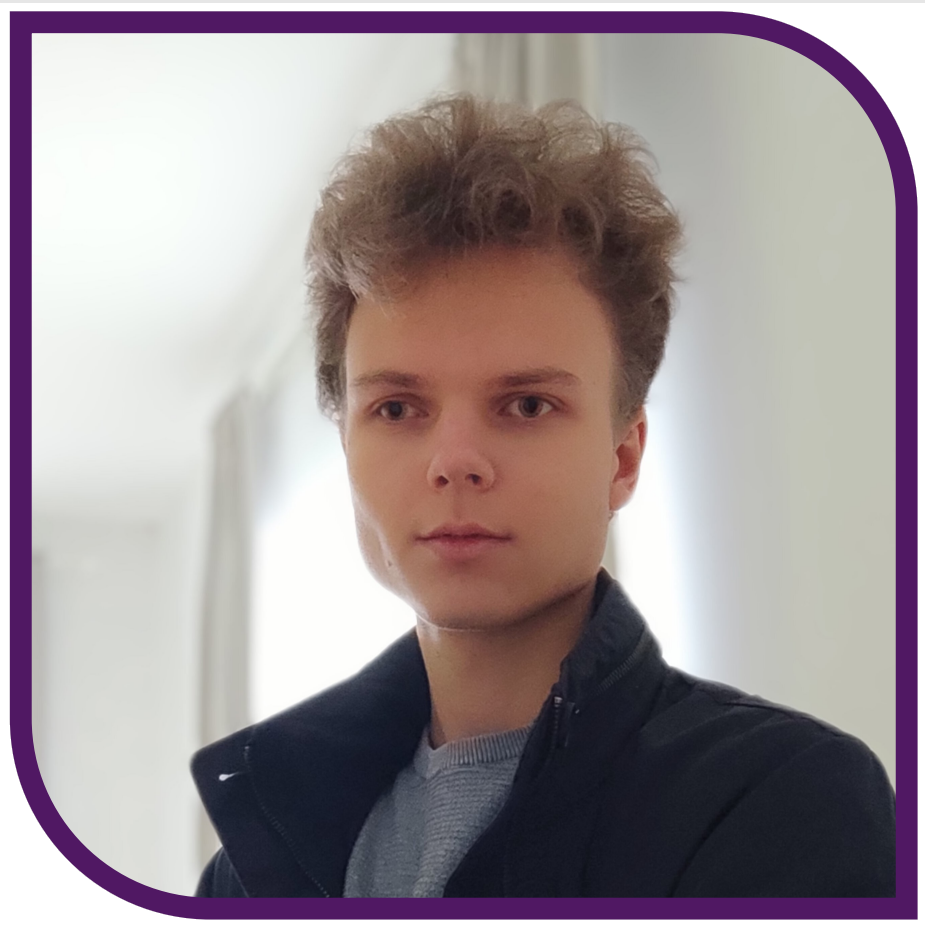
\includegraphics[width=6cm]{images/framed_profile.png}};
\end{tikzpicture}

\name{Hubert Rozmarynowski}
\tagline{Junior Elixir Developer}
 %\photo{2.8cm}{images/profile}
 %\photo[width=0.5\textwidth, right]{6cm}{images/profile}
\personalinfo{%
  % Not all of these are required!
  % You can add your own with \printinfo{symbol}{detail}
  \mailaddress{qwertyqwerty@gmail.com}
  \phone{xxx xxx xxx}
%  \mailaddress{}
  \location{Earth, Milky Way}
%  \homepage{abhinavj004.github.io}
%  \twitter{@marissamayer}
   \newcommand{\githubview}{\href{https://github.com/1hubert}{\color{blue}\faGithubSquare\ \footnotesize {GitHub}}}
   \newcommand{\linkedinview}{\href{https://www.linkedin.com/in/hubert-rozmarynowski/}{\color{blue}{\faLinkedinSquare\ \footnotesize LinkedIn}}}
   \newline{}
   \githubview{}
   \color{elixir} \quad\textbar\quad
   \linkedinview{}
   \newline
  %% You MUST add the academicons option to \documentclass, then compile with LuaLaTeX or XeLaTeX, if you want to use \orcid or other academicons commands.
%   \orcid{orcid.org/0000-0000-0000-0000}
}

%% Make the header extend all the way to the right, if you want. 
%\begin{fullwidth}
\makecvheader
%\end{fullwidth}

%% Depending on your tastes, you may want to make fonts of itemize environments slightly smaller
% \AtBeginEnvironment{itemize}{\small}

\textcolor{black}{\textbf{Lorem ipsum dolor sit amet, consectetur adipiscing elit. Morbi tincidunt orci vel tristique vestibulum. Quisque nulla lectus, condimentum at ultricies dapibus, commodo suscipit leo. Fusce ullamcorper eros nec mattis venenatis. Proin dictum est non aliquam dictum. Fusce lectus arcu, rutrum nec magna a, pharetra efficitur lacus.}}

%% Provide the file name containing the sidebar contents as an optional parameter to \cvsection.
%% You can always just use \marginpar{...} if you do
%% not need to align the top of the contents to any
%% \cvsection title in the "main" bar.

\cvsection[page1sidebar]{Doświadczenie}

\cvevent{Praktyki zawodowe}{ZTM}{Marzec 2021}{Poznań}
\begin{itemize}
\item Praca z dokumentacją techniczną przy diagnostyce sterowników.
\item Wymiana i konserwacja części mechanicznych tramwaju.
\item Komunikacja z pracownikami zespołu: zadawanie jasnych i sprecyzowanych pytań, przyznawanie się do błędów.
\end{itemize}



\cvsection{Projekty}

\cvevent{Symulator Giełdy}{Projekt w ramach kursu}{Sierpień 2022}{}
\begin{itemize}
\item Aplikacja webowa umożliwiająca rejestrację konta użytkownika, kupno i sprzedaż papierów wartościowych, oraz podgląd na swoje portfolio i historię transakcji.
\item Napisana w Pythonie używając micro-frameworka Flask, SQLite do komunikacji z bazą danych i IEX Cloud Legacy API do pobierania rzeczywistych notowań giełdowych.

\end{itemize}
\medskip
\divider

\cvevent{Bandcamp Downloader}{Projekt Samokształceniowy}{Sierpień 2019}{}
\begin{itemize}
    \item Skrypt napisany w Pythonie z biblioteką Selenium WebDriver automatyzujący pobieranie próbkowych wersji utworów muzycznych ze strony Bandcamp.
    \item Do każdego pliku MP3 dodawana jest okładka i metadane.
\end{itemize}
\divider
\medskip

\cvevent{Distraction-Free Matematykaszkolna}{Projekt Samokształceniowy}{Styczeń 2022}{}
\begin{itemize}
    \item Proste rozszerzenie do Chrome usuwające rozpraszające animowane emotki na sprecyzowanej stronie. Napisane w JavaScript.
\end{itemize}

% Adapted from @Jake's answer from http://tex.stackexchange.com/a/82729/226
% \wheelchart{outer radius}{inner radius}{
% comma-separated list of value/text width/color/detail}


\clearpage




%% If the NEXT page doesn't start with a \cvsection but you'd
%% still like to add a sidebar, then use this command on THIS
%% page to add it. The optional argument lets you pull up the 
%% sidebar a bit so that it looks aligned with the top of the
%% main column.
% \addnextpagesidebar[-1ex]{page3sidebar}

\end{document}
